\documentclass[review]{elsarticle}

\usepackage{lineno,hyperref}
\modulolinenumbers[5]
\usepackage{graphicx}
\usepackage{floatrow}
\floatsetup[table]{capposition=top}
\newfloatcommand{capbtabbox}{table}[][\FBwidth]
\usepackage{subfigure}
\graphicspath{{Figures/}}
\usepackage[T1]{fontenc} % optional
\usepackage{amsmath}
\usepackage{epstopdf}
\usepackage{indentfirst}
\usepackage{amsmath}
\usepackage{fancyhdr}
\usepackage{algorithm}
\usepackage{algorithmic}
%\usepackage{multicol}
\usepackage{diagbox}[2011/11/22]
\usepackage{enumerate}
\newcommand{\tabincell}[2]{\begin{tabular}{@{}#1@{}}#2\end{tabular}}% ·ÅÔÚµ¼ÑÔÇø
%\newcommand{\upcite}[1]{\textsuperscript{\cite{#1}}}
\usepackage{multirow}
\usepackage{multirow}
\usepackage[normalem]{ulem}
\usepackage{comment}
\usepackage{threeparttable}
\usepackage{mathrsfs,amsfonts,amssymb}
\useunder{\uline}{\ul}{}
\usepackage{geometry}
\usepackage{rotating}
\floatname{algorithm}{Procedure}
\geometry{top=2.5cm,bottom=3cm}
\newcommand{\upcite}[1]{\textsuperscript{\cite{#1}}}

\usepackage{supertabular}
\usepackage{array}
\usepackage{booktabs} %调整表格线与上下内容的间隔
\usepackage{amsmath} 
\usepackage{amssymb}
\usepackage{longtable}
\usepackage{url}

\usepackage{blindtext}
\usepackage{xparse}%
\usepackage{morewrites}

\usepackage{wrapfig}
\usepackage{xkeyval}%

\newwrite\authorbibfile%

\AtBeginDocument{%
	\immediate\openout\authorbibfile=\jobname.aub%
}%

\AtEndDocument{%
	\immediate\closeout\authorbibfile
	\InputIfFileExists{\jobname.aub}{}{}
}%


\makeatletter

\define@key{authorbib}{scale}[1]{%
	\def\AuthorbibKVMacroScale{#1}%
}

\define@key{authorbib}{wraplines}[10]{%
	\def\AuthorbibKVMacroWraplines{#1}%
}

\define@key{authorbib}{imagewidth}[4cm]{%
	\def\AuthorbibKVMacroImagewidth{#1}%
}

\define@key{authorbib}{overhang}[10pt]{%
	\def\AuthorbibKVMacroOverhang{#1}%
}


\define@key{authorbib}{imagepos}[l]{%
	\def\AuthorbibKVMacroImagepos{#1}%
}

\makeatother

\presetkeys{authorbib}{imagepos=l,imagewidth=4cm,wraplines=15,overhang=20pt}{}

\newlength{\AuthorbibTopSkip}
\newlength{\AuthorbibBottomSkip}
\setlength{\AuthorbibTopSkip}{\baselineskip}
\setlength{\AuthorbibBottomSkip}{\baselineskip}


\NewDocumentCommand{\authorbibliography}{+o+m+m+m}{%
	\IfNoValueTF{#1}{%
	}{%
		\setkeys{authorbib}{#1}%
		\immediate\write\authorbibfile{%
			\string\begin{wrapfigure}[\AuthorbibKVMacroWraplines]{\AuthorbibKVMacroImagepos}[\AuthorbibKVMacroOverhang]{\AuthorbibKVMacroImagewidth}^^J
				\string\includegraphics[scale=\AuthorbibKVMacroScale]{#2}^^J
				\string\end{wrapfigure}^^J
		}%
	}%
	\IfNoValueTF{#3}{%
		\typeout{Warning: No author name}%
	}{%
		\immediate\write\authorbibfile{%
			\unexpanded{\vspace{\AuthorbibTopSkip}}^^J
			\string\noindent\relax
			\unexpanded{\textbf{#3}\par}^^J
			\string\noindent\relax
			\unexpanded{#4}^^J%
			\unexpanded{\vspace{\AuthorbibBottomSkip}}^^J
		}%
	}%
}%
\journal{Journal of \LaTeX\ Templates}

%%%%%%%%%%%%%%%%%%%%%%%
%% Elsevier bibliography styles
%%%%%%%%%%%%%%%%%%%%%%%
%% To change the style, put a % in front of the second line of the current style and
%% remove the % from the second line of the style you would like to use.
%%%%%%%%%%%%%%%%%%%%%%%

%% Numbered
%\bibliographystyle{model1-num-names}

%% Numbered without titles
%\bibliographystyle{model1a-num-names}

%% Harvard
%\bibliographystyle{model2-names.bst}\biboptions{authoryear}

%% Vancouver numbered
%\usepackage{numcompress}\bibliographystyle{model3-num-names}

%% Vancouver name/year
%\usepackage{numcompress}\bibliographystyle{model4-names}\biboptions{authoryear}

%% APA style
%\bibliographystyle{model5-names}\biboptions{authoryear}

%% AMA style
%\usepackage{numcompress}\bibliographystyle{model6-num-names}

%% `Elsevier LaTeX' style
\bibliographystyle{elsarticle-num}
%%%%%%%%%%%%%%%%%%%%%%%

\begin{document}

%\begin{frontmatter}
%
%\title{Elsevier \LaTeX\ template\tnoteref{mytitlenote}}
%\tnotetext[mytitlenote]{Fully documented templates are available in the elsarticle package on \href{http://www.ctan.org/tex-archive/macros/latex/contrib/elsarticle}{CTAN}.}
%
%%% Group authors per affiliation:
%\author{Elsevier\fnref{myfootnote}}
%\address{Radarweg 29, Amsterdam}
%\fntext[myfootnote]{Since 1880.}
%
%%% or include affiliations in footnotes:
%\author[mymainaddress,mysecondaryaddress]{Elsevier Inc}
%\ead[url]{www.elsevier.com}
%
%\author[mysecondaryaddress]{Global Customer Service\corref{mycorrespondingauthor}}
%\cortext[mycorrespondingauthor]{Corresponding author}
%\ead{support@elsevier.com}
%
%\address[mymainaddress]{1600 John F Kennedy Boulevard, Philadelphia}
%\address[mysecondaryaddress]{360 Park Avenue South, New York}
%
%\begin{abstract}
%This template helps you to create a properly formatted \LaTeX\ manuscript.
%\end{abstract}
%
%\begin{keyword}
%\texttt{elsarticle.cls}\sep \LaTeX\sep Elsevier \sep template
%\MSC[2010] 00-01\sep  99-00
%\end{keyword}
%
%\end{frontmatter}
%
%\linenumbers
%
%\section{The Elsevier article class}
%
%\paragraph{Installation} If the document class \emph{elsarticle} is not available on your computer, you can download and install the system package \emph{texlive-publishers} (Linux) or install the \LaTeX\ package \emph{elsarticle} using the package manager of your \TeX\ installation, which is typically \TeX\ Live or Mik\TeX.
%
%\paragraph{Usage} Once the package is properly installed, you can use the document class \emph{elsarticle} to create a manuscript. Please make sure that your manuscript follows the guidelines in the Guide for Authors of the relevant journal. It is not necessary to typeset your manuscript in exactly the same way as an article, unless you are submitting to a camera-ready copy (CRC) journal.
%
%\paragraph{Functionality} The Elsevier article class is based on the standard article class and supports almost all of the functionality of that class. In addition, it features commands and options to format the
%\begin{itemize}
%\item document style
%\item baselineskip
%\item front matter
%\item keywords and MSC codes
%\item theorems, definitions and proofs
%\item lables of enumerations
%\item citation style and labeling.
%\end{itemize}
%
%\section{Front matter}
%
%The author names and affiliations could be formatted in two ways:
%\begin{enumerate}[(1)]
%\item Group the authors per affiliation.
%\item Use footnotes to indicate the affiliations.
%\end{enumerate}
%See the front matter of this document for examples. You are recommended to conform your choice to the journal you are submitting to.
%
%\section{Bibliography styles}
%
%There are various bibliography styles available. You can select the style of your choice in the preamble of this document. These styles are Elsevier styles based on standard styles like Harvard and Vancouver. Please use Bib\TeX\ to generate your bibliography and include DOIs whenever available.
%
%Here are two sample references: \cite{Feynman1963118,Dirac1953888}.
%
%\section*{References}
%
%\bibliography{mybibfile}

%\begin{IEEEbiography}[{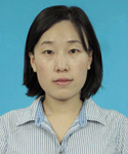
\includegraphics[width=1in,height=1.25in,clip,keepaspectratio]{xiaoyan}}]{Xiaoyan Zhu}
%	received her PhD degree in computer science and technology from Xi'an Jiaotong University, China, in 2013. Currently, she is working as an associate professor in the School of Computer Science and Technology, Xi'an Jiaotong University. Her current research interests include data mining and machine learning.
%\end{IEEEbiography}
%
%% if you will not have a photo at all:
%%\begin{IEEEbiographynophoto}{John Doe}
%%Biography text here.
%%\end{IEEEbiographynophoto}

%\begin{IEEEbiography}[{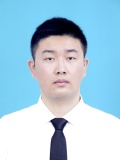
\includegraphics[width=1in,height=1.25in,clip,keepaspectratio]{chenzhen}}]{Chenzhen Ying} received his Bachelor degree in computer science and technology from Xi'an Jiaotong University, China, in 2018. Now, he is a candidate master student in the Department of Computer Science and Technology, Xi'an Jiaotong University. His current research interest is on data mining and machine learning.
%\end{IEEEbiography}
%
%
%\begin{IEEEbiography}[{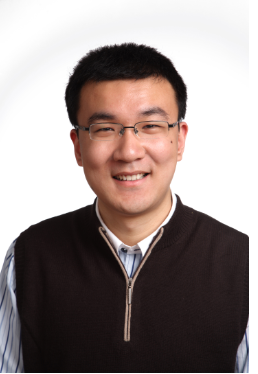
\includegraphics[width=1in,height=1.25in,clip,keepaspectratio]{jiayin}}]{Jiayin Wang}
%	received her PhD degree in computer science and engineering from University of Connecticut, USA, in 2013. Currently, he is working as a professor in the School of Computer Science and Technology, Xi'an Jiaotong University. His current research interests include bioinformatics computing and machine learning.
%\end{IEEEbiography}


%\begin{IEEEbiography}[{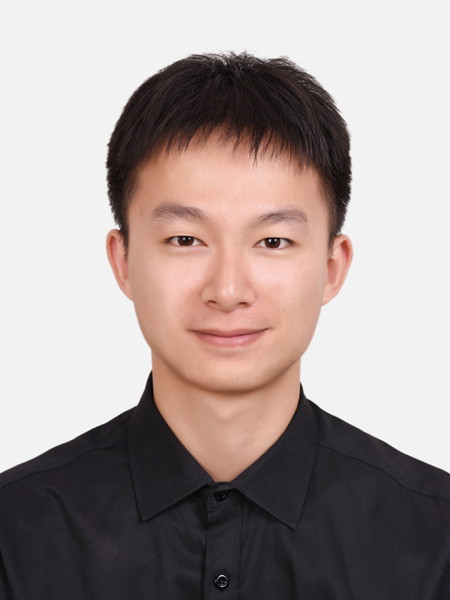
\includegraphics[width=1in,height=1.25in,clip,keepaspectratio]{yingbin}}]{Yingbin Li} received his Bachelor degree from Xi’an Jiaotong University, China, in 2018. Now, he is a candidate master student  in the Department of Computer Science and Technology, Xi’an Jiaotong University. And his current research focus on data mining and machine learning. 
%\end{IEEEbiography}


%\begin{IEEEbiography}[{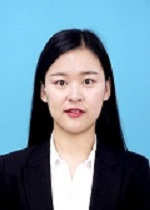
\includegraphics[width=1in,height=1.25in,clip,keepaspectratio]{xiaomei}}]{Xiaomei Yang}
%Yang Xiaomei received her Master degree in computer science and technology from Xi'an Jiaotong University, China, in 2018. Now, she is working in Chang'an University. Her current research interest is on data mining.
%\end{IEEEbiography}



% insert where needed to balance the two columns on the last page with
% biographies
%\newpage

%\begin{biography}[{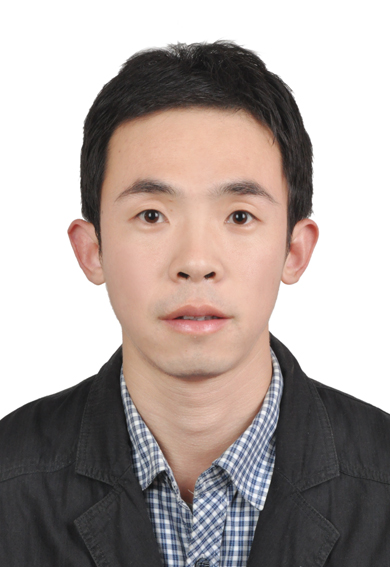
\includegraphics[width=1in,height=1.25in,clip,keepaspectratio]{guangtao}}]{Guangtao Wang}
%	received his PhD degree in computer science and technology from Xi'an Jiaotong University, China, in 2013. He currently is a research fellow in JD AI Research, Mountain View, CA, USA. His research interests include data mining and machine learning.
%\end{biography}


\authorbibliography[scale=0.5,wraplines=5,overhang=40pt,imagewidth=4cm,imagepos=l]{xiaoyan}{Xiaoyan Zhu}{received her PhD degree in computer science and technology from Xi'an Jiaotong University, China, in 2013. Currently, she is working as an associate professor in the School of Computer Science and Technology, Xi'an Jiaotong University. Her current research interests include data mining and machine learning.}

\authorbibliography[scale=2.3,wraplines=5,overhang=40pt,imagewidth=4cm,imagepos=l]{chenzhen}{Chenzhen Ying}{received his Bachelor degree in computer science and technology from Xi'an Jiaotong University, China, in 2018. Now, he is a candidate master student in the Department of Computer Science and Technology, Xi'an Jiaotong University. His current research interest is on data mining and machine learning.}

\authorbibliography[scale=0.4,wraplines=5,overhang=40pt,imagewidth=4cm,imagepos=l]{jiayin}{Jiayin Wang}{received her PhD degree in computer science and engineering from University of Connecticut, USA, in 2013. Currently, he is working as a professor in the School of Computer Science and Technology, Xi'an Jiaotong University. His current research interests include bioinformatics computing and machine learning.}

\authorbibliography[scale=0.6,wraplines=5,overhang=40pt,imagewidth=4cm,imagepos=l]{guangtao}{Guangtao Wang}{received his PhD degree in computer science and technology from Xi'an Jiaotong University, China, in 2013. He currently is a research fellow in JD AI Research, Mountain View, CA, USA. His research interests include data mining and machine learning.}

\end{document}